\documentclass[a4paper, 12pt, UTF8]{article}

\usepackage{xeCJK}
\setCJKmainfont[BoldFont={SimHei},ItalicFont={KaiTi}]{SimSun}

\usepackage{amsfonts}
\usepackage{amsmath}
\usepackage{graphicx}
\usepackage{indentfirst}
\usepackage{listings}
\lstset{
    columns=flexible,
    breakatwhitespace=false,
    breaklines=true,
    frame=single,
    numbers=left,
    numbersep=5pt,
    showspaces=false,
    showstringspaces=false,
    showtabs=false,
    stepnumber=1,
    rulecolor=\color{black},
    tabsize=2,
    texcl=true,
    escapeinside={\%*}{*)},
    extendedchars=false,
    mathescape=true,
}

\usepackage[colorlinks, citecolor=red]{hyperref}

\setlength{\evensidemargin}{-0.05in}
\setlength{\oddsidemargin}{-0.05in}
\setlength{\headheight}{-0.2in}
\setlength{\headsep}{0in}
\setlength{\textheight}{9.75in}
\setlength{\textwidth}{6.5in}
\setlength{\parindent}{2em}

\renewcommand{\baselinestretch}{1.5}

\begin{document}

\title{计算机视觉第1次作业}
\author{黎健成}
\date{2015210936}
\maketitle

%-----
\section{实验目的}

\begin{enumerate}

\item 熟悉RGB、HSV、CIELab颜色空间、直方图。

\item 利用HSV(或RGB,CIELab)颜色直方图,进行基于颜色的图像检索。

\end{enumerate}


\section{实验要求}

\begin{enumerate}

\item 取四张图片,画出三种模型下的颜色直方图。

RGB:各通道256级。

HSV:H通道灰度级180,S通道灰度级256。

CIElab:忽略亮度L通道,并且将a及b通道量化为50个区间。

\item 采用RGB, HSV量化,累加直方图,CCV,Centering refinement,Color Coherence Distance Refinement进行图像检索。

\end{enumerate}

{\large 注意}

\begin{itemize}

\item 相似性度量:采用Correlation、直方图相交Intersection、开方统计Chi-Square statistic、巴式距离Bhattacharyya四种方法进行相似性度量。

\item HSV的区域2分为8个灰度区。

\item 采用OpenCV和Matlab或其它方法均可。

\item 注意颜色空间的转换方式以及图像文件的读取。

\end{itemize}


\section{实验环境}

操作系统:Ubuntu 14.04.3 LTS

(刚开始用Windows 10,然后发现用Python的PIL读取jpg文件时得到的RGB编码与Ubuntu下不同,而bmp文件却是一致的。经测试在Ubuntu下用Python得到jpg文件的RGB编码与mspaint一致,故改用Ubuntu。)

开发环境:Python 2.7.6 + OpenCV 2.4.11

Python Library:

\begin{itemize}

\setlength{\itemsep}{0pt}

\item numpy 1.10.2

\item matplotlib 1.5.0

\item Pillow 3.1.1

\end{itemize}

\section{实验过程}

\subsection{查看不同颜色空间的编码方式}

具体实现见\lstinline[language=bash]{hw1.py的demo1()}。

\begin{enumerate}

\item 给定的彩色JPG图片如图[\ref{figure_1}]。其中,彩色条块的RGB值分别为(255, 0, 0), (0, 255, 0), (0, 0, 255), (255, 0, 0), (0, 255, 0), (0, 0, 255),灰色方块值为(50, 50, 50), (150, 150, 150), (200, 200, 200)。

\begin{figure}[h!]
    \centering
    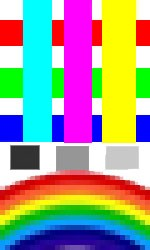
\includegraphics[width=0.2\textwidth]{in/1.jpg}
    \caption{1.jpg}
    \label{figure_1}
\end{figure}

\item 输出RGB颜色空间的通道数值。

如图[\ref{figure_demo1_B}]为B通道的数值。其在红、绿、黄区域的值为0,而在白、蓝、洋红等区域的值为255,在三个灰色方块区域则分别约为50,150,200。

\begin{figure}[h!]
    \centering
    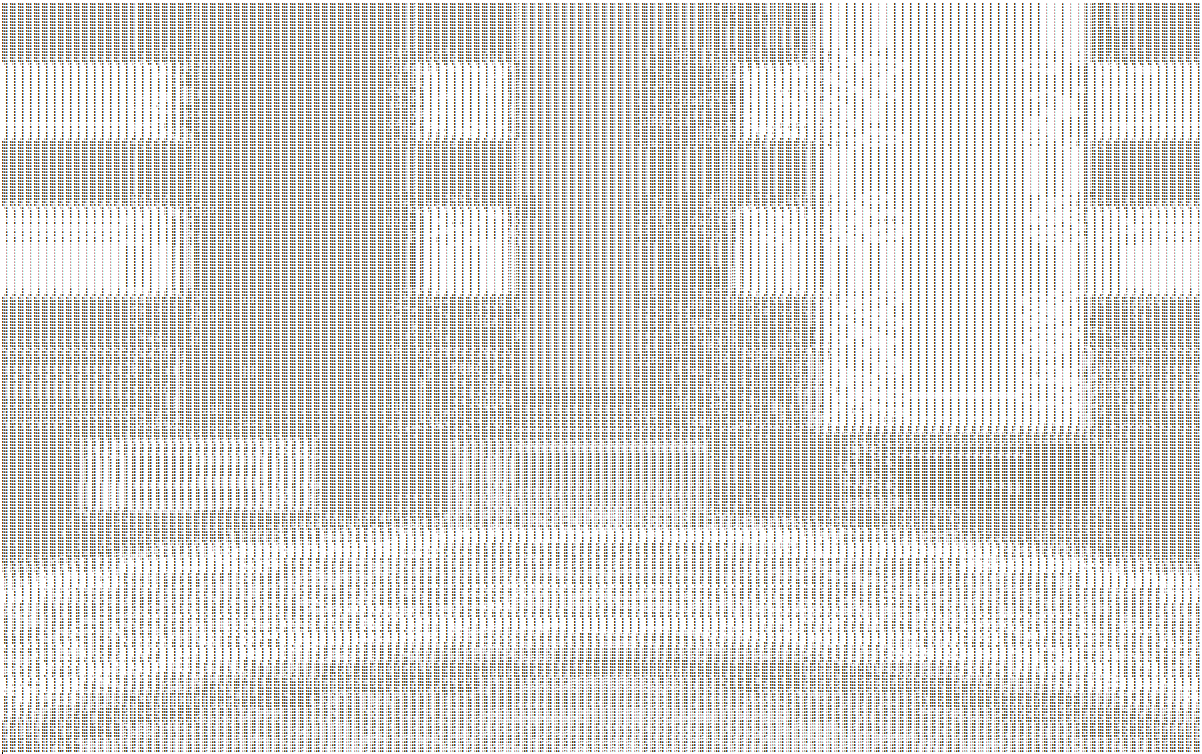
\includegraphics[width=0.8\textwidth]{out/demo1_B.png}
    \caption{B通道的数值}
    \label{figure_demo1_B}
\end{figure}

\item 输出HSV颜色空间的通道数值。

如图[\ref{figure_demo1_H}]为H通道的数值。虽然设计上HSV颜色空间的H通道取值范围是[0, 359],但在OpenCV中,通过自带的cvtColor函数转换的H数值范围为[0, 179]。其原因是测试图像的格式为8UC3,每通道仅8位,最大表示值255,故在存储H通道时其数值均被除以2后保存。如红色区域的值依然为0,绿色区域值则变为90,洋红区域为150等。

\begin{figure}[h!]
    \centering
    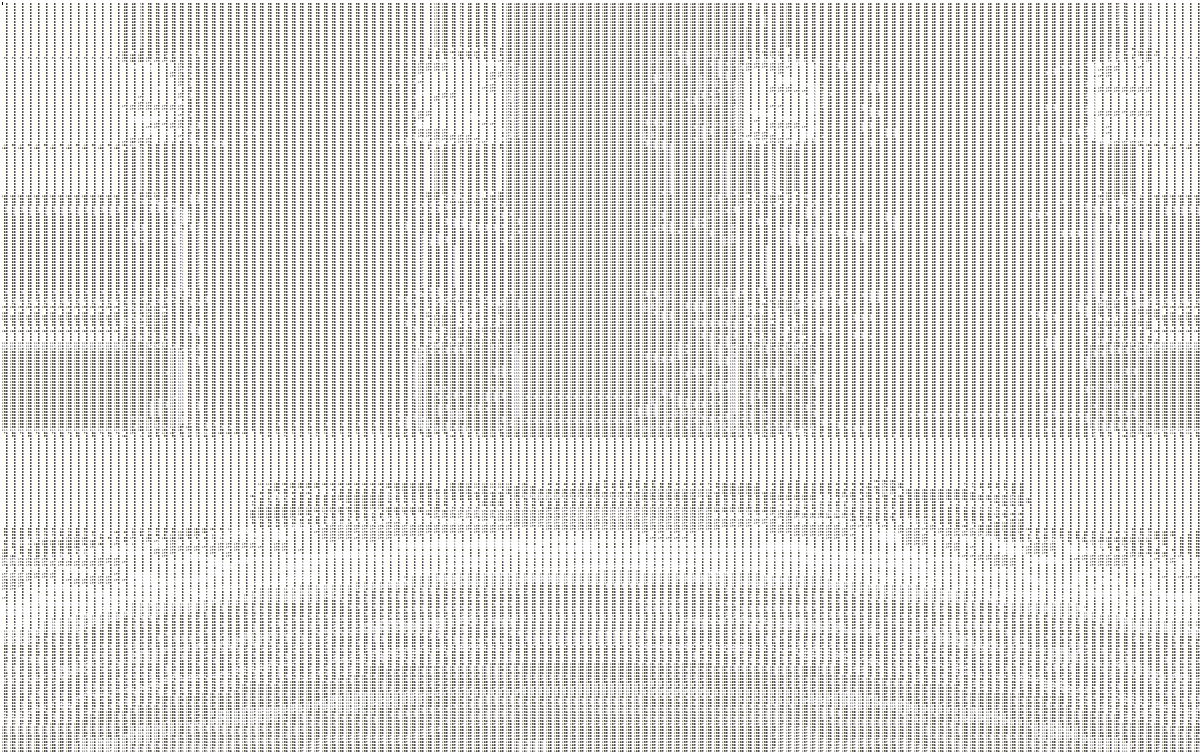
\includegraphics[width=0.8\textwidth]{out/demo1_H.png}
    \caption{H通道的数值}
    \label{figure_demo1_H}
\end{figure}

\item 输出CIELab颜色空间的通道数值。

如图[\ref{figure_demo1_a-}]为a*通道的数值。

\begin{figure}[h!]
    \centering
    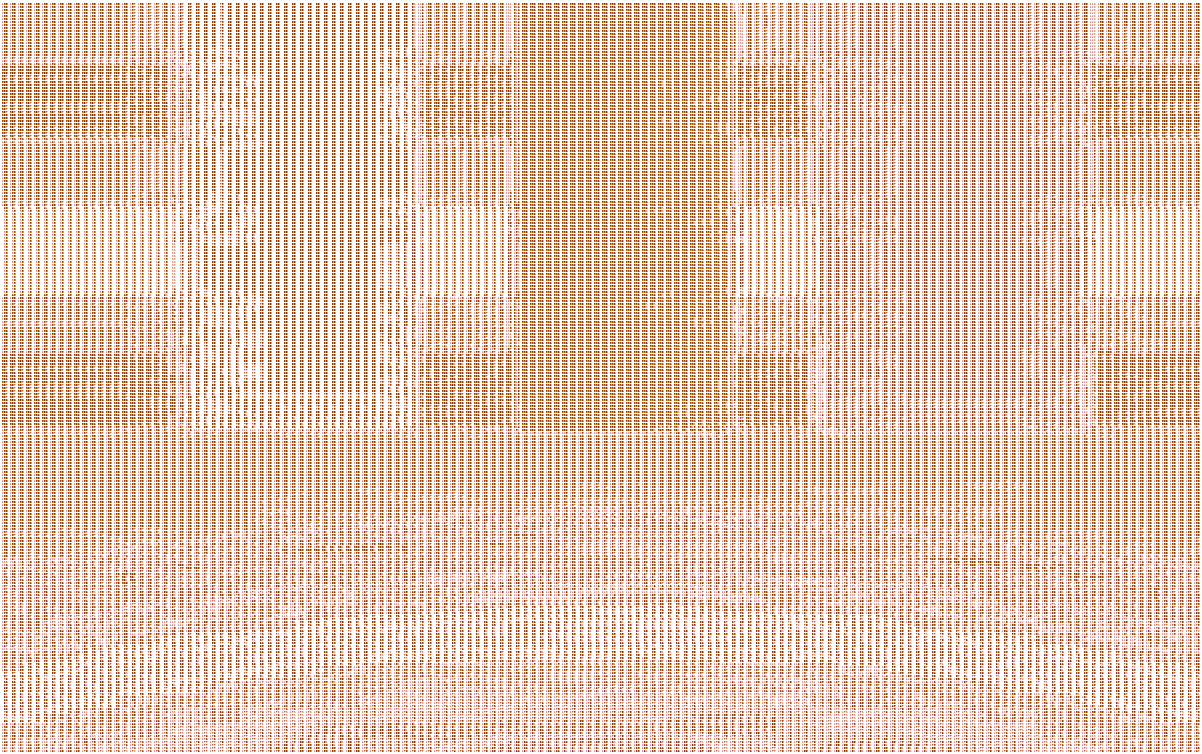
\includegraphics[width=0.8\textwidth]{out/demo1_a-.png}
    \caption{a*通道的数值}
    \label{figure_demo1_a-}
\end{figure}

\end{enumerate}

\clearpage

\subsection{画出不同颜色空间的颜色直方图}

具体实现见\lstinline[language=bash]{hw1.py的demo2()}。

\begin{enumerate}

\item 给定的4张图片如图[\ref{figure_4}]。

\begin{figure}[h!]
    \centering
    \begin{tabular}{cc}
        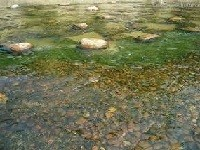
\includegraphics[width=0.3\textwidth]{in/r1.jpg} &
        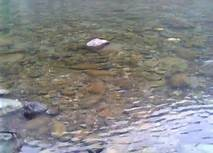
\includegraphics[width=0.3\textwidth]{in/r2.jpg} \\
        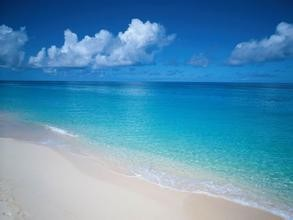
\includegraphics[width=0.3\textwidth]{in/s1.jpg} &
        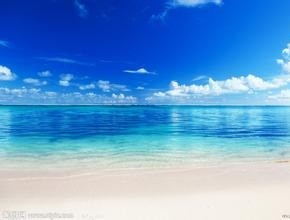
\includegraphics[width=0.3\textwidth]{in/s2.jpg}
    \end{tabular}
    \caption{给定的4张图片}
    \label{figure_4}
\end{figure}

\item 画出RGB颜色空间的颜色直方图。

如图[\ref{figure_demo2_r1_RGB}]为图片r1.jpg在RGB颜色空间各通道256级的颜色直方图。

\begin{figure}[h!]
    \centering
    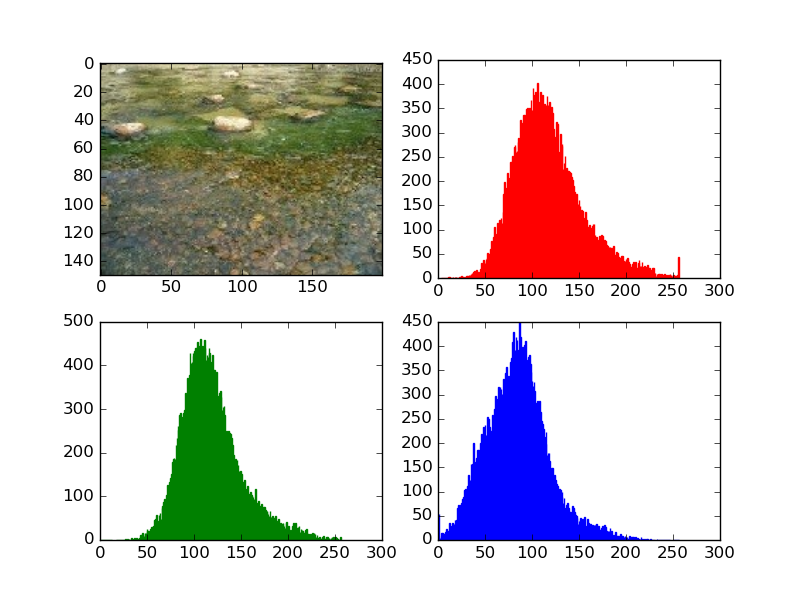
\includegraphics[width=0.7\textwidth]{out/demo2_r1_RGB.png}
    \caption{r1.jpg在RGB颜色空间各通道的颜色直方图}
    \label{figure_demo2_r1_RGB}
\end{figure}

\item 画出HSV颜色空间的颜色直方图。

如图[\ref{figure_demo2_r1_HSV}]为图片r1.jpg在HSV颜色空间各通道的颜色直方图,其中H通道180级,S通道256级。

\begin{figure}[h!]
    \centering
    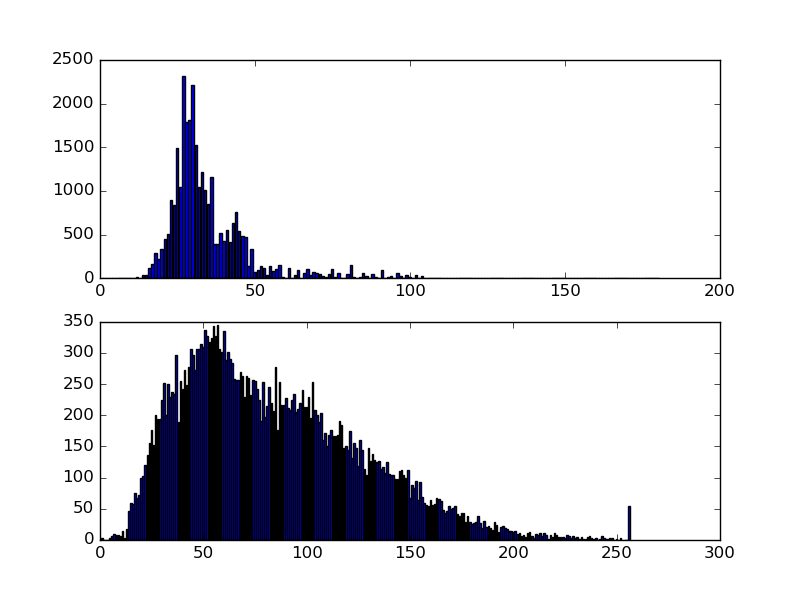
\includegraphics[width=0.7\textwidth]{out/demo2_r1_HSV.png}
    \caption{r1.jpg在HSV颜色空间各通道的颜色直方图}
    \label{figure_demo2_r1_HSV}
\end{figure}

\item 画出HSV颜色空间的颜色直方图。

如图[\ref{figure_demo2_r1_Lab}]为图片r1.jpg在CIELab颜色空间a*和b*通道的颜色直方图,其中忽略亮度L通道,并且将a*及b*通道量化为50个区间。

\begin{figure}[h!]
    \centering
    \includegraphics[width=0.7\textwidth]{out/demo2_r1_Lab.png}
    \caption{r1.jpg在CIELab颜色空间a*和b*通道的颜色直方图}
    \label{figure_demo2_r1_Lab}
\end{figure}

\end{enumerate}


\subsection{相似性度量}

采用Correlation、Intersection、Chi-Square statistic、Bhattacharyya四种方法进行相似性度量。前两者数值越大越相似,后两者数值越小越相似。

比较图片对分别使用r1.jpg自身比较、r1.jpg与r2.jpg、s1.jpg与s2.jpg、r1.jpg与s1.jpg、r2.jpg与s2.jpg。

具体步骤为:读取图片,转换相应的颜色空间,获取直方图并归一化(normalize),使用相似性度量方法计算。

具体实现见\lstinline[language=bash]{hw1.py的demo3()}。

\begin{enumerate}

\item RGB直方图对比

结果如表1-5所示。

\begin{table}[h!]
    \centering
    \caption{r1.jpg, r1.jpg}
    \begin{tabular}{ccccc}
        methods & Correlation & Intersection & Chi-Square & Bhattacharyya \\ \hline
        B通道 & 1.0 & 10.62 & 0.0 & 0.0 \\
        G通道 & 1.0 & 10.12 & 0.0 & 0.0 \\
        R通道 & 1.0 & 10.92 & 0.0 & 0.0 \\
    \end{tabular}
\end{table}
\begin{table}[h!]
    \centering
    \caption{r1.jpg, r2.jpg}
    \begin{tabular}{ccccc}
        methods & Correlation & Intersection & Chi-Square & Bhattacharyya \\ \hline
        B通道 & 0.2889 & 5.064 & 32.18 & 0.5027 \\
        G通道 & 0.7849 & 7.105 & 4.803 & 0.2467 \\
        R通道 & 0.7335 & 7.114 & 4.473 & 0.2891 \\
    \end{tabular}
\end{table}
\begin{table}[h!]
    \centering
    \caption{s1.jpg, s2.jpg}
    \begin{tabular}{ccccc}
        methods & Correlation & Intersection & Chi-Square & Bhattacharyya \\ \hline
        B通道 & 0.5591 & 4.681 & 35.92 & 0.4597 \\
        G通道 & 0.1419 & 7.873 & 271.7 & 0.3835 \\
        R通道 & 0.2032 & 3.495 & 100.3 & 0.4631 \\
    \end{tabular}
\end{table}
\begin{table}[h!]
    \centering
    \caption{r1.jpg, s1.jpg}
    \begin{tabular}{ccccc}
        methods & Correlation & Intersection & Chi-Square & Bhattacharyya \\ \hline
        B通道 & -0.4942 & 1.33 & 399.2 & 0.8178 \\
        G通道 & 0.4537 & 6.986 & 32.23 & 0.3361 \\
        R通道 & -0.3558 & 3.487 & 439.3 & 0.6114 \\
    \end{tabular}
\end{table}
\begin{table}[h!]
    \centering
    \caption{r2.jpg, s2.jpg}
    \begin{tabular}{ccccc}
        methods & Correlation & Intersection & Chi-Square & Bhattacharyya \\ \hline
        B通道 & -0.262 & 2.141 & 43.36 & 0.7489 \\
        G通道 & 0.02588 & 5.089 & 192.7 & 0.4629 \\
        R通道 & -0.1566 & 1.772 & 76.47 & 0.6888 \\
    \end{tabular}
\end{table}

\item HSV直方图对比

结果如表6-10所示。

\begin{table}[h!]
    \centering
    \caption{r1.jpg, r1.jpg}
    \begin{tabular}{ccccc}
        methods & Correlation & Intersection & Chi-Square & Bhattacharyya \\ \hline
        H通道 & 1.0 & 5.177 & 0.0 & 0.0 \\
        S通道 & 1.0 & 11.89 & 0.0 & 0.0 \\
    \end{tabular}
\end{table}
\begin{table}[h!]
    \centering
    \caption{r1.jpg, r2.jpg}
    \begin{tabular}{ccccc}
        methods & Correlation & Intersection & Chi-Square & Bhattacharyya \\ \hline
        H通道 & 0.3443 & 2.764 & 607.4 & 0.6227 \\
        S通道 & 0.365 & 4.133 & 39.05 & 0.5627 \\
    \end{tabular}
\end{table}
\begin{table}[h!]
    \centering
    \caption{s1.jpg, s2.jpg}
    \begin{tabular}{ccccc}
        methods & Correlation & Intersection & Chi-Square & Bhattacharyya \\ \hline
        H通道 & 0.608 & 2.636 & 57.13 & 0.4693 \\
        S通道 & 0.2109 & 4.175 & 14.8 & 0.4123 \\
    \end{tabular}
\end{table}
\begin{table}[h!]
    \centering
    \caption{r1.jpg, s1.jpg}
    \begin{tabular}{ccccc}
        methods & Correlation & Intersection & Chi-Square & Bhattacharyya \\ \hline
        H通道 & -0.1053 & 0.2805 & 605.8 & 0.9074 \\
        S通道 & -0.5593 & 3.497 & 575.5 & 0.6268 \\
    \end{tabular}
\end{table}
\begin{table}[h!]
    \centering
    \caption{r2.jpg, s2.jpg}
    \begin{tabular}{ccccc}
        methods & Correlation & Intersection & Chi-Square & Bhattacharyya \\ \hline
        H通道 & 0.3748 & 2.908 & 12.75 & 0.5823 \\
        S通道 & 0.1554 & 2.094 & 7.748 & 0.6871 \\
    \end{tabular}
\end{table}

\item CIELab直方图对比

结果如表11-15所示。

\begin{table}[h!]
    \centering
    \caption{r1.jpg, r1.jpg}
    \begin{tabular}{ccccc}
        methods & Correlation & Intersection & Chi-Square & Bhattacharyya \\ \hline
        a*通道 & 1.0 & 1.792 & 0.0 & 1.054e-08 \\
        b*通道 & 1.0 & 2.595 & 0.0 & 0.0 \\
    \end{tabular}
\end{table}
\begin{table}[h!]
    \centering
    \caption{r1.jpg, r2.jpg}
    \begin{tabular}{ccccc}
        methods & Correlation & Intersection & Chi-Square & Bhattacharyya \\ \hline
        a*通道 & 0.6671 & 0.9079 & 6.052 & 0.4784 \\
        b*通道 & 0.3151 & 0.841 & 81.75 & 0.6894 \\
    \end{tabular}
\end{table}
\begin{table}[h!]
    \centering
    \caption{s1.jpg, s2.jpg}
    \begin{tabular}{ccccc}
        methods & Correlation & Intersection & Chi-Square & Bhattacharyya \\ \hline
        a*通道 & 0.7837 & 1.675 & 0.5608 & 0.4285 \\
        b*通道 & 0.4061 & 1.465 & 4.474 & 0.5354 \\
    \end{tabular}
\end{table}
\begin{table}[h!]
    \centering
    \caption{r1.jpg, s1.jpg}
    \begin{tabular}{ccccc}
        methods & Correlation & Intersection & Chi-Square & Bhattacharyya \\ \hline
        a*通道 & 0.7133 & 1.23 & 20.19 & 0.392 \\
        b*通道 & -0.07661 & 0.2636 & 29.49 & 0.9078 \\
    \end{tabular}
\end{table}
\begin{table}[h!]
    \centering
    \caption{r2.jpg, s2.jpg}
    \begin{tabular}{ccccc}
        methods & Correlation & Intersection & Chi-Square & Bhattacharyya \\ \hline
        a*通道 & 0.7458 & 1.159 & 7.76 & 0.5482 \\
        b*通道 & 0.5326 & 1.307 & 8.433 & 0.6422 \\
    \end{tabular}
\end{table}

\item RGB累加直方图对比

结果如表16-20所示。

\begin{table}[h!]
    \centering
    \caption{r1.jpg, r1.jpg}
    \begin{tabular}{ccccc}
        methods & Correlation & Intersection & Chi-Square & Bhattacharyya \\ \hline
        B通道 & 1.0 & 13.92 & 0.0 & 0.0 \\
        G通道 & 1.0 & 12.62 & 0.0 & 0.0 \\
        R通道 & 1.0 & 12.8 & 0.0 & 0.0 \\
    \end{tabular}
\end{table}
\begin{table}[h!]
    \centering
    \caption{r1.jpg, r2.jpg}
    \begin{tabular}{ccccc}
        methods & Correlation & Intersection & Chi-Square & Bhattacharyya \\ \hline
        B通道 & 0.9124 & 11.26 & 1.998 & 0.1944 \\
        G通道 & 0.9833 & 11.61 & 0.5281 & 0.08815 \\
        R通道 & 0.9788 & 11.58 & 0.7862 & 0.1178 \\
    \end{tabular}
\end{table}
\begin{table}[h!]
    \centering
    \caption{s1.jpg, s2.jpg}
    \begin{tabular}{ccccc}
        methods & Correlation & Intersection & Chi-Square & Bhattacharyya \\ \hline
        B通道 & 0.9226 & 6.896 & 2.097 & 0.2329 \\
        G通道 & 0.9734 & 11.36 & 1.691 & 0.09031 \\
        R通道 & 0.9617 & 14.75 & 1.02 & 0.0554 \\
    \end{tabular}
\end{table}
\begin{table}[h!]
    \centering
    \caption{r1.jpg, s1.jpg}
    \begin{tabular}{ccccc}
        methods & Correlation & Intersection & Chi-Square & Bhattacharyya \\ \hline
        B通道 & 0.6379 & 7.311 & 6.941 & 0.4102 \\
        G通道 & 0.9498 & 11.08 & 0.6977 & 0.08537 \\
        R通道 & 0.8906 & 11.57 & 734.5 & 0.2704 \\
    \end{tabular}
\end{table}
\begin{table}[h!]
    \centering
    \caption{r2.jpg, s2.jpg}
    \begin{tabular}{ccccc}
        methods & Correlation & Intersection & Chi-Square & Bhattacharyya \\ \hline
        B通道 & 0.651 & 5.721 & 7.104 & 0.4684 \\
        G通道 & 0.926 & 10.59 & 18.15 & 0.1711 \\
        R通道 & 0.8738 & 10.21 & 3.336e+03 & 0.368 \\
    \end{tabular}
\end{table}

\item CCV对比

CCV即颜色聚合向量(Color Coherence Vector)\textsuperscript{\cite{ref1}},主要作用是将颜色簇划分成聚合(coherence)和非聚合(incoherent),以此来解决颜色直方图无法表达图像色彩的空间位置的缺点。

根据论文\cite{ref2},这里使用L1距离来比较两张图像RGB颜色空间的CCV,且对给定的4张图像进行两两比较。

结果如表21所示。

\begin{table}[h!]
    \centering
    \caption{CCV-L1距离对比}
    \begin{tabular}{ccccc}
         & r1 & r2 & s1 & s2 \\ \hline
        r1 & 0 & 27403 & 93222 & 93434 \\ \hline
        r2 & 27403 & 0 & 77551 & 89939 \\ \hline
        s1 & 93222 & 77551 & 0 & 76586 \\ \hline
        s2 & 93434 & 89939 & 76586 & 0 \\ \hline
    \end{tabular}
\end{table}

\item Centering Refinement

Centering Refinement \textsuperscript{\cite{ref2}},指对图像的颜色直方图中的每个像素,把它分为在图像中心的和不在图像中心的两个部分。在图像中心指在图像中心$75\%$的区域中。最后再使用L1距离来比较两张图像经过Centering Refinement的直方图。

为了方便,这里使用中心$64\%$的区域作为中心区域,即上下左右各$10\%$的区域不为中心区域。同样,这里对给定的4张图像RGB颜色空间进行两两比较。

结果如表22所示。

\begin{table}[h!]
    \centering
    \caption{Centering Refinement Histogram-L1距离对比}
    \begin{tabular}{ccccc}
         & r1 & r2 & s1 & s2 \\ \hline
        r1 & 0 & 30961 & 91068 & 93438 \\ \hline
        r2 & 30961 & 0 & 76685 & 89519 \\ \hline
        s1 & 91068 & 76685 & 0 & 76064 \\ \hline
        s2 & 93438 & 89519 & 76064 & 0 \\ \hline
    \end{tabular}
\end{table}

\item Color Coherence Distance Refinement

Color Coherence Distance Refinement指论文\cite{ref2}中的Successive Refinement,即以上两种方法的结合:对每个像素根据聚合和中心分为4类。

结果如表23所示。

\begin{table}[h!]
    \centering
    \caption{Color Coherence Distance Refinement-L1距离对比}
    \begin{tabular}{ccccc}
         & r1 & r2 & s1 & s2 \\ \hline
        r1 & 0 & 33463 & 93234 & 93438 \\ \hline
        r2 & 33463 & 0 & 81319 & 90079 \\ \hline
        s1 & 93234 & 81319 & 0 & 84790 \\ \hline
        s2 & 93438 & 90079 & 84790 & 0 \\ \hline
    \end{tabular}
\end{table}

\end{enumerate}


\subsection{基于颜色的图像检索}

基于颜色的图像检索,属于基于内容的图像检索——即CBIR(Content-based image retrieval)。具体来说,指用户输入一张图片,查找某个图片集中具有相同或相似颜色特征的其他图片。

这里使用RGB颜色直方图、HSV量化后的颜色直方图、RGB颜色累加直方图、CCV、Centering Refinement、Color Coherence Distance Refinement这6种方法进行图像检索。其中,前三种方法分别使用Correlation、Intersection、Chi-Square statistic、Bhattacharyya4种方法进行相似性度量,后三种方法使用L1距离进行相似性度量。

由于图片集只有r1.jpg, r2.jpg, s1.jpg, s2.jpg、r1.jpg与s1.jpg、r2.jpg与s2.jpg这4张图片,故这里对每张图片、每种方法都检索一张图片,并以表格的形式呈现结果。

具体实现见\lstinline[language=bash]{hw1.py的demo4()}。

结果如表24所示。

\begin{table}[h!]
    \centering
    \caption{CBIR}
    \begin{tabular}{ccccccc}
        method & compare_method & r1 & r2 & s1 & s2 \\ \hline
        RGB直方图    & Correlation   & r2 & r1 & s2 & s1 \\ \hline
        RGB直方图    & Intersection  & r2 & r1 & s2 & s1 \\ \hline
        RGB直方图    & Chi-Square    & r2 & s2 & r2 & s1 \\ \hline
        RGB直方图    & Bhattacharyya & r2 & r1 & s2 & s1 \\ \hline
        HSV量化直方图 & Correlation   & r2 & r1 & s2 & s1 \\ \hline
        HSV量化直方图 & Intersection  & r2 & r1 & r2 & s1 \\ \hline
        HSV量化直方图 & Chi-Square    & s1 & s2 & s2 & r2 \\ \hline
        HSV量化直方图 & Bhattacharyya & r2 & r1 & s2 & s1 \\ \hline
        RGB累加直方图 & Correlation   & r2 & r1 & s2 & s1 \\ \hline
        RGB累加直方图 & Intersection  & r2 & r1 & s2 & s1 \\ \hline
        RGB累加直方图 & Chi-Square    & r2 & r1 & s2 & s1 \\ \hline
        RGB累加直方图 & Bhattacharyya & r2 & r1 & s2 & s1 \\ \hline
        CCV         & L1            & r2 & r1 & s2 & s1 \\ \hline
        CR          & L1            & r2 & r1 & s2 & s1 \\ \hline
        CCDR        & L1            & r2 & r1 & r2 & s1 \\ \hline
    \end{tabular}
\end{table}

观察表格知,大部分方法都能得到较好的结果。

纵向比较知,

对r1.jpg,只有HSV量化直方图+Chi-Square没有得到最相似图片。

对r2.jpg,只有RGB和HSV量化直方图+Chi-Square都没有得到最相似图片。

对s1.jpg,则是RGB直方图+Chi-Square、HSV量化直方图+Intersection、CCDR+L1没有得到最相似图片。

对s2.jpg,只有HSV量化直方图+Chi-Square没有得到最相似图片。

横向比较知,

HSV量化直方图+Chi-Square效果最不好。Chi-Square相对其它方法效果没那么好,HSV量化直方图没有RGB直方图效果好,累加直方图的效果比直方图好。

CCDR则没有达到论文所说效果,在s1.jpg中没有得到最相似图片。

\section{实验结论}

从实验结果分析知,对颜色组成基本一致的图像,如两张大海的图像,使用直方图方法判断相似度的结果更能符合人的判断。而对两张河流的图片,虽然图像内容同样都是河水、鹅卵石,因在颜色组成上有较大差异,使用直方图的判断效果不佳。

3种颜色空间和4种相似性度量方法各有差异,可以考虑在进行比较时综合考虑4种方法。CCV、Centering refinement、Color Coherence Distance Refinement也有各自的优点。

通过这次实验,熟悉了颜色表示的方式,对使用直方图等方法判断颜色相似度也有一定的了解,实现了简单的基于颜色的图像检索,达到了实验目的。


\renewcommand{\refname}{参考}
\begin{thebibliography}{9}
\bibitem{ref1} 颜色聚合向量. 百度百科. 最后修订于2014年11月15日. \url{http://baike.baidu.com/view/4913318.htm}
\bibitem{ref2} Pass G, Zabih R. Histogram refinement for content-based image retrieval[C]//Applications of Computer Vision, 1996. WACV'96., Proceedings 3rd IEEE Workshop on. IEEE, 1996: 96-102.
\end{thebibliography}

\end{document}